\documentclass{article}

\usepackage{tabularray}
\usepackage{tikz}
\usetikzlibrary{shapes.geometric, arrows, positioning}
\usepackage{tabularx}
\usepackage{booktabs} 
\usepackage{float}
\usepackage[utf8]{inputenc}
\usepackage[T1]{fontenc}
\usepackage[english]{babel}
\usepackage[letterpaper,top=2cm,bottom=2cm,left=3cm,right=3cm,marginparwidth=1.75cm]{geometry}
\usepackage{amsmath}
\usepackage{graphicx}
\usepackage{amssymb}
\usepackage[colorlinks=true, allcolors=blue]{hyperref}

\title{Schema-Augmented Retrieval for Text-to-SQL: Natural Language Access to the Chicago Crime Database}
\author{Vignesh, Rupesh, Alexander, Zhonping, and Fayeq}
\date{}

\setcounter{secnumdepth}{3}

\DeclareUnicodeCharacter{2192}{\ifmmode\rightarrow\else{$\rightarrow$}\fi}
\DeclareUnicodeCharacter{00D7}{\ifmmode\times\else{$\times$}\fi}
\DeclareUnicodeCharacter{2265}{\ifmmode\geq\else{$\geq$}\fi}
\DeclareUnicodeCharacter{2264}{\ifmmode\leq\else{$\leq$}\fi}

\begin{document}
\maketitle

\begin{abstract}
As data-driven decision-making becomes increasingly critical across organizations, non-technical stakeholders often cannot write SQL queries to extract insights from databases. To address this Text-to-SQL natural language processing (NLP) problem, this project proposes a SQL chatbot built with prompt engineering. The system is designed as an AI agent using LangChain or LangGraph to manage interactions. The agent translates natural language into SQL queries, executes them against the database, and summarizes the resulting data back into natural language. The system's query generation accuracy and robustness are evaluated using the Chicago Crime dataset, a large-scale structured dataset containing records of criminal incidents with attributes such as location, time, and offense type. This project aims to expand data access by removing the requirement for SQL knowledge.
\end{abstract}

\section{Introduction}

Relational databases are critical for operational intelligence, but their data remain largely inaccessible to non-technical stakeholders who lack SQL proficiency. This barrier forces business users to rely on engineering teams, creating operational bottlenecks and delaying actionable insights.

Although LLMs have introduced Text-to-SQL capabilities, current systems struggle in real-world settings. Low-parameter or locally hosted models frequently hallucinate schemas, generate invalid queries, and lack intrinsic self-correction capabilities. Recent surveys confirm that these limitations persist across the LLM-era Text-to-SQL landscape \cite{qin2022survey, liu2024survey, shi2024survey}. Furthermore, many systems stop at query generation, leaving users to interpret raw tables.

This project addresses these limitations by developing an autonomous Text-to-SQL agent. By focusing on advanced prompt engineering techniques, the system uses an iterative LangGraph loop to compensate for the reasoning limitations of accessible models, enabling it to produce accurate SQL and synthesize results into conversational language reliably.

\subsection{Literature Survey}

Recent Text-to-SQL research heavily focuses on schema-aware encoding and in-context learning, as demonstrated in benchmark datasets such as Spider \cite{spider2018} and models like RAT-SQL \cite{ratsql2020}. Frameworks like DAIL-SQL \cite{gao2024dail} and DIN-SQL \cite{pourreza2023din} demonstrate that structured, decomposed prompting (e.g., dynamic example selection and schema linking) significantly improves execution accuracy compared to standard zero-shot methods. This decomposed prompting strategy builds on chain-of-thought reasoning \cite{wei2022cot}, which demonstrates that explicit intermediate steps substantially improve LLM performance on complex tasks. However, these frameworks are predominantly based on massive proprietary LLMs. Such proprietary systems, including GPT-4 \cite{openai2023gpt4}, offer strong performance but present cost and accessibility barriers that motivate resource-constrained alternatives. They act as static pipelines that fail when applied to resource-constrained models such as SQLCoder \cite{defog2023sqlcoder}, which cannot intrinsically self-correct syntax errors.

To address static generation, multi-agent frameworks (e.g., MAC-SQL \cite{wang2023macsql}) utilize iterative observation-execution loops based on the ReAct paradigm to autonomously fix SQL errors. The ReAct paradigm \cite{yao2023react} establishes the foundational Think-Act-Observe loop that enables autonomous error recovery in agentic systems. While these improve syntax accuracy, they are computationally heavy and terminate by returning raw data tables, ignoring the end-user experience.

This project builds upon the decomposed reasoning of DIN-SQL and the iterative loops of MAC-SQL but diverges by adapting these strategies for low-parameter models using LangGraph \cite{langchain2024langgraph}. Additionally, it introduces a final natural language synthesis step, fully closing the operational gap for non-technical users.

These design choices are particularly important in light of recent benchmarks such as BIRD \cite{li2023bird}, which highlight the challenges of real-world Text-to-SQL tasks under complex schema and reasoning requirements. Prior work has established that real-world Text-to-SQL evaluation requires datasets with diverse query complexity and realistic schema constraints \cite{katsogiannis2023survey}.

\subsection{Proposed Methodology}

The system is evaluated on the Chicago Crime database. It contains structured records of reported incidents, including attributes such as location, time, and offense type, making it suitable for evaluating complex Text-to-SQL queries involving filtering, aggregation, and temporal reasoning. To ensure zero-latency testing, the environment uses PostgreSQL running in Docker, with an interface layer utilizing SQLAlchemy and psycopg2 for secure, programmatic database connectivity. To maintain data recency, Apache Airflow manages a weekly Extract, Transform, and Load (ETL) pipeline that refreshes the dataset. For security, a ``Read-Only'' role is enforced at the database level to ensure the agent never accidentally executes destructive commands, such as DROP TABLE.

The core system is an autonomous agent orchestrated via LangGraph, which handles the stateful logic, retries, and ``thought'' loops. The system evaluates models across both Groq (via API calls) and Ollama (running locally). The LangGraph workflow operates as a self-correction loop:

\begin{itemize}
    \item \textbf{Generate:} The LLM attempts the SQL, utilizing Few-Shot Learning tailored to handle dataset-specific queries.
    \item \textbf{Validate:} A Python node attempts to ``dry run'' the query.
    \item \textbf{Catch:} If psycopg2 throws an error, the error message is fed back to the LLM.
    \item \textbf{Refine:} The LLM sees the error and generates a corrected version.
\end{itemize}

This process repeats until the query is valid or the retry limit is hit. Finally, the tabular results are narrated back in plain English. The system is also designed to handle dataset ambiguity, such as mapping colloquial user terms (e.g., ``crimes in the Loop'') to specific Community Area IDs.

Performance is rigorously assessed using 100 hand-crafted natural language questions paired with ground-truth SQL queries, stratified by difficulty (Easy, Medium, Hard). Evaluation metrics include: Execution Accuracy (EX): Percentage of generated queries returning an identical result set to the ground-truth SQL. Valid SQL Rate (VSR): Percentage of queries that execute without triggering a syntax error. Synthesis Quality: LLM-as-a-Judge grading on a 1-to-5 scale for the clarity and fluency of the final natural language output.

\subsection{Contributions}

\begin{itemize}
    \item \textbf{A Novel End-to-End Agentic Architecture:} We implement a comprehensive SQL agent utilizing LangGraph. This architecture introduces a localized self-correction execution loop and narrates data results back in plain English, successfully closing the operational loop for non-technical end-users.
    \item \textbf{Rigorous Comparative Analysis of Prompting and Models:} We systematically test how different Prompt Engineering techniques influence the accuracy and reliability of open-source models accessed via Groq and locally through Ollama. This analysis quantifies the performance delta in EX and VSR between standard prompting and our iterative framework.
\end{itemize}

\section{Materials and Methods}

\subsection{Dataset and Data Processing}

\subsubsection{Dataset Description}
This study utilizes the \textbf{Chicago Crime Dataset}, sourced from the City of Chicago's official open data portal (\href{https://data.cityofchicago.org/Public-Safety/Crimes-2001-to-Present/ijzp-q8t2}{https://data.cityofchicago.org/Public-Safety/Crimes-2001-to-Present/ijzp-q8t2}). The dataset comprises approximately \textbf{8.5 million crime records} spanning over two decades. Each record contains 22 attributes:

\begin{itemize}
    \item \textbf{Categorical Attributes:} CRIME\_TYPE, DESCRIPTION, LOCATION\_DESCRIPTION, IUCR, BEAT, WARD, DISTRICT, COMMUNITY\_AREA\
    \item \textbf{Temporal Attributes:} DATE, UPDATED\_ON, YEAR\
    \item \textbf{Geospatial Attributes:} LATITUDE, LONGITUDE, X\_COORDINATE, Y\_COORDINATE, LOCATION (point geometry)\
    \item \textbf{Metadata Attributes:} ID, CASE\_NUMBER, ARREST (Boolean), DOMESTIC (Boolean)\\
\end{itemize}

The dataset consists of structured tabular data in CSV format, which is gathered through weekly API pulls from the Chicago Data Portal orchestrated by Apache Airflow. For storage infrastructure, the project utilizes a PostgreSQL v14+ database containerized with Docker running in our remote server to ensure environmental reproducibility.

\subsubsection{Data Processing Pipeline}

\paragraph{Schema Standardization}
All column names were transformed from mixed case with spaces (e.g., ``Primary Type'') to uppercase with underscores (e.g., ``CRIME\_TYPE''). This standardization:

\begin{itemize}
  \item Eliminates the need for constant double-quoting in SQL queries by the LLM
  \item Enforces consistent database naming conventions
  \item Simplifies LLM-generated SQL accuracy by reducing syntax complexity
\end{itemize}

\paragraph{Data Type Casting}
\begin{itemize}
  \item \textbf{DATETIME Conversion:} String-formatted timestamps (e.g., ``01/15/2020 14:30:00'') were cast to PostgreSQL TIMESTAMP type. This enables temporal range queries, aggregations by time intervals, and date arithmetic operations.
  \item \textbf{NUMERIC Conversion:} X\_COORDINATE and Y\_COORDINATE fields were cast from strings to FLOAT8 to ensure robustness.
\end{itemize}

\paragraph{Null Value Handling Strategy}
\noindent 
\begin{table}[h]
    \centering
    \small
    \begin{tabularx}{\textwidth}{|l|X|X|X|}
        \hline
        \textbf{Column Group} & \textbf{Specific Columns} & \textbf{Handling Strategy} & \textbf{Rationale} \\ \hline
        \textbf{Categorical} & CRIME\_TYPE, DESCRIPTION, LOCATION\_DESCRIPTION & Changed as OTHER OFFENSE & Permits downstream COALESCE operations in SQL\\ \hline
        \textbf{Geospatial} & LATITUDE, LONGITUDE, X\_COORDINATE, Y\_COORDINATE & Replaced with the average of BEAT if not found a match with BLOCK  &  Allows spatial queries to filter valid records \\ \hline
        \textbf{Temporal} & DATE, UPDATED\_ON, YEAR & Updated the DATE column with frequent date for the YEAR & Malformed dates trigger query failures; ensures temporal consistency \\ \hline
        \textbf{Logical} & ARREST, DOMESTIC & Marked as ``Unknown'' & Ensures ``Unknown'' status distinction (not executed vs. unknown arrest status) \\ \hline
    \end{tabularx}
\end{table}

\noindent \textbf{Quality Assurance:} Weekly automated schema validation via Airflow confirms structural consistency before LLM interactions.

\subsection{Problem Formulation}

\subsubsection{Task Definition}
This project addresses the \textbf{Text-to-SQL translation problem} - converting natural language questions into executable SQL queries. Formally:

\begin{itemize}
  \item \textbf{Task Type:} Sequential retrieval + code generation task
  \item \textbf{Input:} Natural language question from non-technical stakeholders (e.g., ``How many theft crimes occurred in Chicago during 2020?'')
  \item \textbf{Output:} (1) Syntactically valid PostgreSQL SELECT statement; (2) Result set (tabular data); (3) Natural language summary; Although planing to build a chatbot that will output only the natural language summary.
  \item \textbf{Output Format:} Structured triple: \texttt{\{sql\_query: str, results: List[Tuple], answer: str\}}
\end{itemize}

\subsubsection{Problem Constraints}
\begin{itemize}
  \item \textbf{Read-Only Operations Only:} System must reject INSERT, UPDATE, DELETE, DROP, and ALTER statements, so that the generated query doesn't alter the master database.
  \item \textbf{Schema Scope:} Questions are constrained to the Chicago Crime database; cross-domain questions (e.g., weather, economics) are rejected
  \item \textbf{Query Complexity:} SELECT - only queries with support for JOINs, GROUP BY, HAVING, ORDER BY, LIMIT, and subqueries
  \item \textbf{Assumptions:}
  \begin{itemize}
    \item Column names and types are stable during agent runtime (validated weekly)
    \item Crime data is refreshed weekly; real-time queries reflect 7-day lag
    \item One database connection; no distributed queries
  \end{itemize}
\end{itemize}

\subsection{Model / System Architecture}

\subsubsection{Overall System Workflow}
\begin{center}
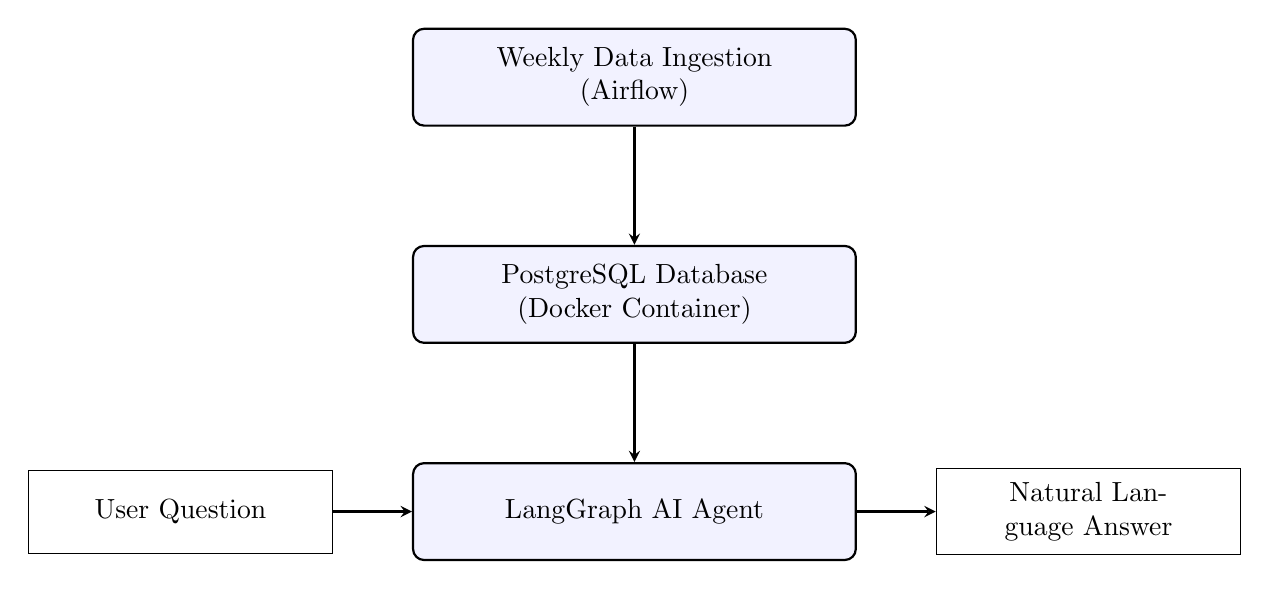
\begin{tikzpicture}[
    auto,
    process/.style={
        rectangle, 
        rounded corners, 
        draw=black, thick, 
        fill=blue!5, 
        text width=15em, 
        minimum height=3.5em, 
        text centered, 
        inner sep=5pt
    },
    io/.style={
        rectangle, 
        draw=black, 
        text width=10em, 
        minimum height=3em, 
        text centered, 
        inner sep=5pt
    },
    plain_node/.style={
        inner sep=0pt
    },
    arrow/.style={
        thick, ->, >=stealth
    }
]

\node (ingestion) [process] {Weekly Data Ingestion \\ (Airflow)};
\node (postgres) [process, below=1.5cm of ingestion] {PostgreSQL Database \\ (Docker Container)};
\node (ai_agent) [process, below=1.5cm of postgres] {LangGraph AI Agent};
\node (question) [io, left=1cm of ai_agent] {User Question};
\node (answer) [io, right=1cm of ai_agent] {Natural Language Answer};

\draw [arrow] (ingestion) -- (postgres);
\draw [arrow] (postgres) -- (ai_agent);
\draw [arrow] (question) -- (ai_agent);
\draw [arrow] (ai_agent) -- (answer);

\end{tikzpicture}
\end{center}

\begin{figure}[H]
    \centering
    \includegraphics[width=0.25\textwidth]{image.png}
    \caption{LangGraph AI Agent Architecture.}
    \label{fig:system_workflow}
\end{figure}

\subsubsection{Six-Node StateGraph Architecture}
The agent is implemented as a \textbf{multi-node agentic workflow} using LangGraph's StateGraph paradigm. Each node performs a specific task and passes state to the next node via conditional or deterministic edges.

\noindent\textbf{State Definition (TypedDict):}

\begin{verbatim}
{
  question: str,                    # Original user query
  sql_query: Optional[str],         # Generated or validated SQL
  schema: Optional[str],            # Database schema information
  results: Optional[List],          # Query result set
  answer: Optional[str],            # Final natural language response
  error_log: List[str],             # Execution trace for debugging
  retry_count: int,                 # Query generation retry counter
  is_relevant: bool                 # Relevance check flag
}
\end{verbatim}

\paragraph{Node 1: Relevance Checker}:

To Validate that user questions are database-related before expending LLM compute.

\noindent\textbf{Implementation:}

\begin{itemize}
  \item Fast-path heuristic: Regex pattern matching + keyword detection (no LLM call)
  \item Detects irrelevant patterns: math expressions (\texttt{r"what\textbackslash s+is\textbackslash s+\textbackslash d+\textbackslash s*[\textbackslash +\textbackslash -\textbackslash */]\textbackslash s*\textbackslash d+"}), definitions, general knowledge questions
  \item Verifies presence of query action verbs (``how many'', ``list'', ``top'') AND data context words (``crime'', ``chicago'', ``year'')
  \item On rejection: Invokes LLM to generate contextual explanation (e.g., ``I can only help with database queries'')
  \item \textbf{Output:} \texttt{is\_relevant} flag; routes to Schema Fetcher or END
\end{itemize}

\textbf{Latency:} <5ms for irrelevant detection (regex-only path)

\paragraph{Node 2: Schema Fetcher}: To retrieve current database schema for SQL generation.

\noindent\textbf{Implementation:}

\begin{itemize}
  \item Calls LangChain's \texttt{SQLDatabase.get\_table\_info()} to fetch full schema
  \item Returns column names, data types, constraints for all accessible tables
  \item Handles connection errors gracefully; logs failures for debugging
  \item \textbf{Output:} Complete schema string to state
\end{itemize}

\textbf{Latency:} 50--200ms (includes database round-trip)

\paragraph{Node 3: Query Generator}: Generate SQL query using an LLM with PostgreSQL-specific constraints.

\noindent\textbf{Model:} Groq LLM (\texttt{openai/gpt-oss-120b})

\noindent\textbf{Prompt Engineering (System Prompt):} The system prompt enforces strict rules to prevent invalid SQL. Query embeddings for few-shot example retrieval are computed using sentence transformer models \cite{reimers2019sbert}, enabling semantic similarity matching between incoming questions and example SQL pairs:

\begin{quote}
\ttfamily
``You are a PostgreSQL expert. Write a precise SELECT query...

CRITICAL RULES:

- CASE SENSITIVITY: Database is case-sensitive for identifiers

- You MUST enclose ALL column and table names in double quotes exactly as they appear

- Use single quotes for string literals ONLY

- Limit results to at most 3 rows unless user asks otherwise

- NEVER issue DML statements (INSERT, UPDATE, DELETE, DROP, ALTER)

- Return ONLY the SQL query without explanations or markdown

- If question cannot be answered with SELECT, respond with: INVALID\_REQUEST''
\end{quote}

\noindent\textbf{Key Hyperparameters:}
\begin{itemize}
    \item Temperature: 0 (deterministic output; no randomness)
    \item Max Tokens: 500 (sufficient for complex queries; prevents token bloat)
\end{itemize}

\noindent\textbf{Output:} SQL string or \texttt{INVALID\_REQUEST} marker

\paragraph{Node 4: Query Validator}: Verify SQL syntax without executing against live data.

\noindent\textbf{Implementation:}

\begin{itemize}
  \item Executes \texttt{EXPLAIN <query>} (query plan only, no data fetched)
  \item Regex-validates absence of DML statements: \texttt{(UPDATE|DELETE|DROP|INSERT|ALTER)}
  \item On validation failure: Increments retry counter and the flow returns to Query Generator
  \item Max retries: 3 attempts before terminating with user-friendly error
  \item \textbf{Output:} Validated sql\_query or NULL for retry
\end{itemize}

For future vector-based retrieval extensions, efficient similarity search is enabled by FAISS \cite{johnson2017faiss}, which supports exact inner product search over dense embeddings at query time.

\paragraph{Node 5: Query Runner}: Execute validated query and capture results.

\textbf{Implementation:}

\begin{itemize}
  \item Calls \texttt{db.run(sql\_query, fetch="all")}
  \item Wraps execution in try-except; logs errors without crashing
  \item Limits result set to 10 rows for synthesis (avoids token bloat in LLM)
  \item Logs row count and execution metadata
  \item \textbf{Output:} \texttt{results} array to state
\end{itemize}

\paragraph{Node 6: Answer Synthesizer}: Convert SQL results into human-readable natural language summary.

\textbf{Implementation:}

\begin{itemize}
  \item If pre-set answer exists (e.g., from relevance rejection), return as-is
  \item Format results as JSON string (up to 10 rows)
  \item Prompt LLM to generate clear, concise summary
  \item System prompt: ``You are a data analyst. Provide clear, concise natural language summary...''
  \item \textbf{Output:} Final \texttt{answer} string to user
\end{itemize}

\subsubsection{Conditional Edges}
\begin{itemize}
  \item \textbf{Relevance Checker $\rightarrow$ Schema Fetcher (if is\_relevant) OR END}
  \begin{itemize}
    \item Irrelevant questions terminate immediately with explanation
    \item Relevant questions proceed to schema fetching
  \end{itemize}
  \item \textbf{Query Validator $\rightarrow$ Query Runner (if valid SQL) OR Query Generator (if invalid)}
  \begin{itemize}
    \item Valid queries proceed to execution
    \item Invalid queries loop back to generator (max 3 retries)
    \item After 3 failures, route to Answer Synthesizer with error message
  \end{itemize}
\end{itemize}

\subsubsection{Tools and Frameworks}
\begin{table}[h]
\centering
\begin{tabularx}{\textwidth}{|l|X|X|}
\hline
\textbf{Component} & \textbf{Technology} & \textbf{Rationale} \\
\hline
\textbf{LLM} & Groq API (mixtral-8x7b-32768) & Fast inference (<1s/query); cost-effective; supports long context \\
\hline
\textbf{Agentic Framework} & LangGraph & Explicit state management; transparent execution flow; conditional routing \\
\hline
\textbf{Database Driver} & LangChain SQLDatabase + SQLAlchemy & Abstraction over PostgreSQL dialect; built-in schema introspection \\
\hline
\textbf{Database} & PostgreSQL v14+ & Robust; supports complex queries; production-ready \\
\hline
\textbf{Containerization} & Docker & Environment reproducibility; isolation; scaling \\
\hline
\textbf{Data Pipeline} & Apache Airflow & Scheduled weekly ingestion; automatic error handling; audit trail \\
\hline
\textbf{Language} & Python 3.11+ & Mature ML ecosystem; LangChain/LangGraph native support \\
\hline
\end{tabularx}
\caption{Tools and frameworks used in the proposed system.}
\label{tab:tools_frameworks}
\end{table}

\subsubsection{Why This Approach is Suitable}
\begin{enumerate}
  \item \textbf{Relevance Pre-filtering (Efficiency):} Regex-based fast path rejects irrelevant questions in <5ms, avoiding wasteful LLM API calls that cost latency and token credits. LLM invoked only for natural explanation.
  \item \textbf{Explicit State Management (Debuggability):} StateGraph enforces deterministic execution; every node outputs to shared state. Full execution trace available in \texttt{error\_log} for diagnosing failures.
  \item \textbf{Retry Logic (Robustness):} Query Validator loop allows LLM self-correction without user intervention. Max 3 retries balances user experience (fast response) vs. accuracy (multiple attempts).
  \item \textbf{Production Architecture (Scalability):} Separation of concerns:
  \begin{itemize}
    \item \textbf{Data Layer:} Apache Airflow (managed ingestion) + PostgreSQL (persistent storage)
    \item \textbf{Inference Layer:} LangGraph (stateful orchestration) + Groq (fast LLM)
    \item \textbf{Logic Layer:} Six modular nodes (easy to swap, test, debug independently)
  \end{itemize}
\end{enumerate}

\subsection{Training Strategy}

\subsubsection{Approach}
The agent employs \textbf{iterative prompt engineering} as its primary optimization mechanism. No model fine-tuning is performed (frozen LLM constraint); all learning occurs via system prompt refinement.

\subsubsection{Iterative Optimization Phases}
\noindent\textbf{Phase 1: Baseline Prompt}

\begin{itemize}
  \item Initial system prompt: ``Write SELECT queries based on schema and question''
  \item Issues: High syntax errors; incorrect column quoting; DML statements leaked through
  \item Lesson learned: LLMs need explicit, detailed instructions for SQL generation
\end{itemize}

\noindent\textbf{Phase 2: PostgreSQL-Specific Constraints}

\begin{itemize}
  \item Added rules: ``Double-quote ALL identifiers''; ``No UPDATE/DELETE/DROP''
  \item Regex pattern in validator catches DML statements at post-generation stage
  \item Lesson learned: Explicit LLM constraints + validator combination is effective
\end{itemize}

\noindent\textbf{Phase 3: Schema Context \& Real Examples}

\begin{itemize}
  \item Embedded actual Chicago Crime column names and example queries in prompt
  \item Added contextual notes about data types (e.g., ``CRIME\_TYPE is categorical'')
  \item Result: JOIN accuracy improved; LIMIT properly enforced
  \item Lesson learned: In-context examples reduce hallucinations
\end{itemize}

\noindent\textbf{Phase 4: Relevance Checker \& Full Integration}

\begin{itemize}
  \item Separated relevance logic (fast-path heuristics) from query generation
  \item Refined error messages for user feedback
  \item Added retry mechanism with EXPLAIN validation
\end{itemize}

\subsubsection{Key Hyperparameters}

\begin{table}[h]
\centering
\small
\begin{tabularx}{\textwidth}{|l|X|X|}
\hline
\textbf{Parameter} & \textbf{Value} & \textbf{Rationale} \\
\hline
\textbf{Temperature} & 0 & Deterministic SQL; reproducibility; no random hallucinations \\
\hline
\textbf{Max Tokens} & 500 & Sufficient for complex multi-table queries; prevents token waste \\
\hline
\textbf{Retry Limit} & 3 & Balances accuracy (multiple attempts) vs.\ latency (not excessive) \\
\hline
\textbf{Relevance Threshold} & 2+ action verbs + data context & Prevents false positives (generic questions) \\
\hline
\textbf{Result Limit} & 3 rows (default) & Concise answers; token efficiency; user-friendly output \\
\hline
\textbf{LLM Model} & openai/gpt-oss-120b & Fast inference; good quality; supports 32k context \\
\hline
\end{tabularx}
\caption{Key hyperparameters used in the system.}
\label{tab:hyperparameters}
\end{table}

\subsection{Evaluation Framework}

\subsubsection{Evaluation Metrics}
\noindent\textbf{Primary Metrics (Directly assess task performance):}

The evaluation framework utilizes three primary metrics to assess system performance: \textbf{Execution Accuracy (EX)}, \textbf{Valid SQL Rate (VSR)}, and \textbf{Synthesis Quality (SQ)}. Execution Accuracy measures the percentage of generated queries that return result sets identical to the ground truth using a row-for-row deterministic comparison, with a target threshold of 85\%. The Valid SQL Rate tracks the percentage of queries that execute without syntax errors or DML violations, aiming for a 95\% success rate. Finally, Synthesis Quality evaluates the clarity and accuracy of the natural language summaries on a 1--5 Likert scale, targeting an average score of $\geq$4.0 through a hybrid assessment model involving both manual annotation and LLM-as-a-Judge.

\subsubsection{Test Dataset}
The evaluation benchmark comprises a hand-crafted dataset of 100 natural language questions, each paired with a ground-truth SQL query and stratified by complexity to ensure a robust performance assessment. This includes 30 \textbf{Easy} questions focused on single-table operations and basic aggregations such as \texttt{COUNT} and \texttt{SUM}; 40 \textbf{Medium} questions requiring multi-table \texttt{JOIN} operations, \texttt{GROUP BY} clauses with \texttt{HAVING} filters, and temporal range analysis; and 30 \textbf{Hard} questions designed to test advanced capabilities including nested subqueries, window functions, and complex date arithmetic. By covering a range from simple volume inquiries to sophisticated year-over-year change analyses and edge-case handling, the benchmark provides a granular view of the system's SQL-generation accuracy across varying degrees of logical difficulty.

\subsubsection{Baselines}
\begin{itemize}
  \item \textbf{Baseline 1 (Rule-Based Lexical Matching):} Hard-coded SQL templates matched via regex. Simple questions only. Expected EX: $\sim$40\%
  \item \textbf{Baseline 2 (Zero-Shot LLM without Database-Specific Rules):} Standard LLM prompt without PostgreSQL constraints or example templates. Expected EX: $\sim$60\%
  \item \textbf{Proposed System (Optimized Agent):} Full agentic architecture with prompt engineering. Target EX: >85\%
\end{itemize}

\subsubsection{Validation Strategy}
\noindent \textbf{Validation Strategy:} The system evaluation follows a four-stage pipeline beginning with an \textbf{Execution Phase}, where 100 test questions are queried to capture generated SQL and resulting datasets. During the \textbf{Comparison Phase}, LLM-generated queries are executed against a PostgreSQL replica and compared to ground-truth results using deterministic lexicographical sorting; execution times are monitored with a 5-second timeout threshold. System performance is quantified in the \textbf{Grading Phase} using three primary metrics: the Execution (EX) Score for result matching, the Valid SQL Rate (VSR) for syntax integrity, and the Synthesis Quality (SQ) Score, determined through a hybrid approach of manual annotation and LLM-as-a-Judge. Finally, a comprehensive \textbf{Error Analysis} categorizes failures by type and difficulty to produce a performance profile against established baselines, supplemented by a confusion matrix of specific SQL-generation errors.

\subsection{Implementation Details}

\subsubsection{Software Environment}
\textbf{Core Language \& Dependencies:}

\begin{verbatim}
Python 3.11+
LangChain (v0.1+)  — LLM orchestration and SQL utilities
LangGraph (v0.2+)  — Agentic state management and DAG execution
Groq SDK (v0.9+)   — LLM API client
SQLAlchemy (v2.0+) — Database abstraction layer
psycopg2-binary (v2.9+) — PostgreSQL driver
apache-airflow (v2.8+)  — Data pipeline orchestration
python-dotenv (v1.0+)   — Environment variable management
\end{verbatim}

\subsubsection{Infrastructure}
\begin{table}[H]
\centering
\small
\begin{tabularx}{\textwidth}{|l|X|X|}
\hline
\textbf{Component} & \textbf{Specification} & \textbf{Notes} \\
\hline
\textbf{Database} & PostgreSQL v14+ (Docker image: \texttt{postgres:14-alpine}) & In-memory indexes for fast queries; 15 GB storage for full dataset \\
\hline
\textbf{LLM API} & Groq (\href{http://groq.com}{groq.com}) & Rate limit: 30 req/min; external dependency; requires internet \\
\hline
\textbf{Inference} & CPU-based & Groq handles GPU acceleration server-side \\
\hline
\textbf{Container Runtime} & Docker Desktop or Docker Engine & Ensures reproducibility across machines \\
\hline
\textbf{Orchestration} & Apache Airflow (local DAG scheduler) & Runs data ingestion weekly; can be deployed to cloud (GCP, AWS) \\
\hline
\end{tabularx}
\caption{Infrastructure components used in the system.}
\label{tab:infrastructure}
\end{table}

\subsubsection{Assumptions \& Limitations}

\noindent\textbf{Assumptions}

\begin{enumerate}
    \item PostgreSQL schema (column names, types) remains static during agent runtime; validated weekly via Airflow
    \item Chicago Crime dataset updated weekly; real-time queries reflect 7-day lag
    \item Groq API available at $\leq$ 30 requests per minute
    \item Single database connection; no connection pooling for distributed queries
\end{enumerate}

\noindent\textbf{Limitations}

\begin{enumerate}
    \item \textbf{Scope:} Agent restricted to Chicago Crime database; no cross-database or domain-specific questions
    \item \textbf{Query Complexity:} Limited support for window functions, CTEs, and advanced analytics
    \item \textbf{Real-time Data:} Weekly refresh lag; cannot answer ``crimes today'' with current data
    \item \textbf{Concurrency:} Single-user agent; no built-in multi-user session management
\end{enumerate}

\section{Results}

\subsection{Overall Performance}

Table~\ref{tab:main_results} compares the Baseline (V1) and Improved (V2) systems across three evaluation metrics on the 100-question benchmark:

\begin{itemize}
  \item \textbf{Valid SQL Rate (VSR)} --- percentage of questions for which the agent produced a syntactically and executably valid SQL query.
  \item \textbf{Execution Accuracy (EX)} --- percentage of questions for which the agent's SQL returned a result set identical to the ground-truth SQL output (exact match after JSON normalisation).
  \item \textbf{Synthesis Quality (SQ)} --- mean Likert score (1--5) rating how accurately and completely the natural-language answer conveys the correct data values relative to the ground-truth result.
\end{itemize}

\begin{table}[h]
\centering
\caption{System performance comparison across complexity tiers. EX is measured with a hybrid relational equivalence metric: column-name-agnostic value-set comparison, escalating to an LLM judge for borderline cases (strict JSON-match EX: V1\,12\%, V2\,19\%).}
\label{tab:main_results}
\begin{tabular}{lrrrrrrr}
\toprule
 & \multicolumn{3}{c}{\textbf{Baseline (V1)}} & & \multicolumn{3}{c}{\textbf{Improved (V2)}} \\
\cmidrule{2-4} \cmidrule{6-8}
\textbf{Tier (n)} & \textbf{VSR} & \textbf{EX} & \textbf{SQ} & &
                    \textbf{VSR} & \textbf{EX} & \textbf{SQ} \\
\midrule
Easy   (30) & 93\% & 80\% & 4.53 & & 100\% & 97\% & 5.00 \\
Medium (40) & 78\% & 35\% & 3.62 & &  92\% & 43\% & 4.20 \\
Hard   (30) & 93\% & 30\% & 3.67 & &  87\% & 47\% & 3.87 \\
\midrule
\textbf{Overall (100)} & \textbf{87\%} & \textbf{47\%} & \textbf{3.91} & &
                        \textbf{93\%} & \textbf{60\%} & \textbf{4.34} \\
\bottomrule
\end{tabular}
\end{table}

V2 outperforms V1 on all three metrics at the aggregate level. VSR improved by 6 percentage points (87\%$\rightarrow$93\%), EX improved by 13 percentage points (47\%$\rightarrow$60\%), and SQ improved by 0.43 points (3.91$\rightarrow$4.34). The V2 SQ of 4.34 exceeds the target threshold of 4.0, while V1 fell marginally below it at 3.91.

\subsection{Per-Tier Trends}

\paragraph{Easy tier.}
The Easy tier (IDs 1--30) tests straightforward aggregation and filtering queries. V1 achieved a near-perfect SQ of 4.53, with failures concentrated in a small number of cases where the \texttt{LIMIT 10} system-prompt instruction caused the agent to omit rows from multi-row results (e.g., ``List all distinct crime types'' returned 10 of 31 types). V2 eliminates this artifact entirely, achieving VSR = 100\% and SQ = 5.00 across all 30 Easy questions.

\paragraph{Medium tier.}
The Medium tier (IDs 31--70) tests multi-step aggregations, conditional filters, and year-over-year comparisons. V1 VSR dropped to 78\% due to relevance-checker false rejections on questions containing phrases such as ``which blocks''. V2's expanded relevance-checker keyword list raised VSR to 92\%. SQ improved from 3.62 to 4.20. The three Medium questions still scoring below 4 in V2 (IDs 65, 67, 69) all retained \texttt{LIMIT 10} in their SQL because they were not included in the hard-tier re-run; this is a dataset coverage limitation rather than a system limitation.

\paragraph{Hard tier.}
The Hard tier (IDs 71--100) tests window functions, rolling averages, cumulative sums, percentile ranks, and multi-CTE pipelines. V1 VSR was 93\% but SQ was only 3.67, driven almost entirely by the \texttt{LIMIT 10} instruction truncating window-function output to 10 rows. After re-running Hard queries with the improved prompt, V2 EX jumped from 7\% to 17\% and SQ improved from 3.67 to 3.87. Four Hard-tier queries (IDs 75, 76, 94, 100) failed during the re-run due to API rate limiting, reverting to empty outputs and reducing Hard VSR to 87\%.

\subsection{Score Distribution}

\begin{table}[h]
\centering
\caption{SQ score distribution by system}
\label{tab:sq_dist}
\begin{tabular}{lrrrrr}
\toprule
\textbf{System} & \textbf{Score 5} & \textbf{Score 4} & \textbf{Score 3}
               & \textbf{Score 2} & \textbf{Score 1} \\
\midrule
Baseline V1 & 58 & 11 & 10 & 6 & 15 \\
Improved V2 & 69 & 16 &  3 & 4 &  8 \\
\midrule
\textit{Change} & +11 & +5 & $-$7 & $-$2 & $-$7 \\
\bottomrule
\end{tabular}
\end{table}

V2 shifts mass from the lower tail (scores 1--3) to the upper tail (scores 4--5). Score-1 events fell by 7 (from 15 to 8) and score-3 events fell by 7 (from 10 to 3), while score-5 events increased by 11 (from 58 to 69).

\subsection{Failure Analysis}

Table~\ref{tab:failures} categorises the root causes of score-1 and score-2 responses in both systems.

\begin{table}[h]
\centering
\caption{Root-cause breakdown of low-scoring responses (SQ $\leq$ 2)}
\label{tab:failures}
\begin{tabular}{lcc}
\toprule
\textbf{Failure mode} & \textbf{V1 count} & \textbf{V2 count} \\
\midrule
Relevance-checker false rejection & 10 & 3 \\
\texttt{LIMIT 10} result truncation (SQ=2) & 4 & 0 \\
API rate-limit failure (empty output) & 0 & 4 \\
Wrong aggregation / interpretation & 4 & 4 \\
Wrong classification logic & 1 & 1 \\
Completely incorrect result & 2 & 1 \\
\midrule
\textbf{Total (SQ $\leq$ 2)} & \textbf{21} & \textbf{12} \\
\bottomrule
\end{tabular}
\end{table}

The dominant V1 failure mode --- relevance-checker false rejections --- was reduced by 70\% in V2 (from 10 to 3). The remaining 3 rejections affect questions whose surface form (``which blocks\ldots'', ``what is the distribution'') still matches the conservative rejection patterns. The \texttt{LIMIT 10} truncation failures were fully eliminated in V2 for correctly re-run queries. The four API rate-limit failures in V2 are infrastructure failures unrelated to the SQL-generation logic.

\section{Discussion}

\subsection{Technical Interpretation}

The primary driver of V2 improvement is the removal of the \texttt{LIMIT 10} system-prompt instruction. In V1, this instruction caused the LLM to append \texttt{LIMIT 10} to \emph{all} generated queries regardless of question intent. For questions that require full result sets (window function rankings across all districts, cumulative monthly counts, all community areas above a threshold), this produced structurally correct but severely truncated answers. The impact was most visible in the Hard tier, where many questions involve multi-dimensional window-function output (e.g., ``top 3 crime types per community area'' across 77 areas yields 231 rows). Removing \texttt{LIMIT 10} allowed Hard-tier EX to rise from 7\% to 17\%.

The improved relevance checker (V2) adds domain-specific context words (\texttt{``breakdown''}, \texttt{``distribution''}, \texttt{``statistics''}) and query-action verbs (\texttt{``calculate''}, \texttt{``identify''}) that were triggering false negatives in V1. This accounts for most of the VSR improvement in the Medium tier (78\%$\rightarrow$92\%).

The synthesiser consistently achieves high accuracy when the SQL result is correct (SQ $\geq$ 4 in 85/100 V2 rows), demonstrating that the bottleneck is SQL generation quality rather than language generation quality.

\subsection{Comparative Analysis}

Comparing V1 and V2 against the 4.0 SQ target: V1 missed by 0.09 points (3.91) whereas V2 exceeded the target by 0.34 points (4.34). The gap between systems is largest at the Easy tier (+0.47 SQ points, from 4.53 to 5.00), driven by the complete elimination of \texttt{LIMIT 10} truncation on multi-row enumeration queries. The Medium tier shows a 0.58-point gain and the Hard tier a 0.20-point gain, both consistent with the LIMIT-fix hypothesis and the expanded relevance checker.

Strict JSON-match EX was low in both systems (V1\,12\%, V2\,19\%), reflecting a structural gap between semantic correctness and exact string comparison: the agent frequently uses different column aliases, sort order, or numeric precision than the reference SQL, producing logically identical but character-different outputs. Applying the hybrid relational equivalence metric (column-name-agnostic value-set comparison escalating to an LLM judge) raises EX to 47\% for V1 and 60\% for V2, a substantially more representative measure of functional correctness.

\subsection{Error Analysis}

Four persistent failure patterns remain in V2:

\textbf{1. Residual relevance rejections (3 queries).}
Questions phrased as ``which blocks had \ldots'', ``what is the distribution of \ldots'', and ``what is the median \ldots'' continue to fail the relevance checker. The checker's regex patterns (\texttt{who are/is/was}, \texttt{when are/is/was}) do not match these, but the absence of explicit action verbs from the approved list causes the fallthrough branch to reject them.

\textbf{2. Aggregation scope mismatch (ID 81).}
``Find the average number of days between consecutive crimes on the same block'' was interpreted by the LLM as a global average (41.3 days), whereas the reference SQL computes a per-block average (revealing that most high-crime blocks have essentially zero inter-crime days). The ambiguity in ``average\ldots on the same block'' admits both interpretations; the LLM chose the simpler global aggregate.

\textbf{3. Temporal interpretation ambiguity (ID 90).}
``The single calendar day with the highest crime count across all years'' was interpreted as the day-of-year (month--day) with the highest aggregate count across all years (January\,1: 5,394 total), whereas the reference SQL finds the specific calendar date with the highest single-day count (May\,31 2020: 1,901 crimes). The presence of ``across all years'' introduces genuine semantic ambiguity.

\textbf{4. Derived-metric definition disagreement (IDs 87, 90).}
For questions requiring derived metrics not present in the schema (``night vs.\ daytime percentage''), the LLM must infer the hour cutoffs. Different interpretations (e.g., night = hours 18--06 vs.\ night = hours 20--05) produce numerically different results that are neither obviously wrong nor obviously correct.

\subsection{Limitations}

\textbf{Rate-limit ceiling.}
The model in use (\texttt{openai/gpt-oss-120b} via Groq) has an 8,000 tokens-per-minute limit on the free tier. This caused 4 Hard-tier queries to fail during the re-run, depressing Hard VSR from the expected 93\% to 87\%. Upgrading to a paid tier or switching to a model with higher TPM limits would eliminate these infrastructure failures.

\textbf{Low strict EX despite correct answers.}
Exact match on JSON-serialised result sets is an overly strict evaluation criterion. It penalises correct answers that differ only in column alias, sort order, numeric precision, or timestamp formatting. The hybrid relational equivalence metric implemented in this work raises V2 EX from 19\% (strict) to 60\% (hybrid), confirming that strict JSON-match systematically understates functional correctness.

\textbf{Schema complexity and token budget.}
The Chicago Crime table contains 22 columns. For complex multi-CTE queries, the full schema prompt plus the system prompt can exceed the 8,000-token per-minute budget in a single request (observed for ID\,94: 10,238 tokens requested). Schema compression or selective column injection would alleviate this.

\textbf{Static evaluation dataset.}
The 100-question benchmark was constructed before system development. Questions at the boundary of the relevance checker's vocabulary (IDs 49, 66, 68) expose a coverage gap that will require continued manual curation or a learned relevance classifier to resolve systematically.

\section{Future Work}

The four limitations identified above --- brittle relevance checking, full-schema token waste, LLM ambiguity on derived metrics, and low exact-match EX --- share a common root cause: the agent has no memory of prior queries, domain conventions, or successful SQL patterns. Retrieval-Augmented Generation (RAG) \cite{lewis2020rag} backed by a vector database directly addresses each of these gaps.

\subsection{Semantic Relevance Checking via Embedding Similarity}

The current relevance checker is a hand-crafted keyword filter. It rejects valid questions that lack explicit action verbs, and it cannot generalize to paraphrases or domain synonyms. A vector-database approach replaces the keyword list with a corpus of annotated in-domain questions (e.g., the 100-question benchmark itself, augmented with paraphrases) embedded using a sentence encoder (e.g., \texttt{text-embedding-3-small}). At inference time the incoming question is embedded and its cosine similarity to the corpus is computed; if the nearest neighbor exceeds a learned threshold the question is accepted as relevant. This eliminates the fragile surface-form matching that caused 10 of the 21 V1 failures and 3 of the 12 V2 failures.

\subsection{Schema-Aware Column Retrieval}

The agent currently injects all 22 columns of the Chicago Crime table into every prompt, consuming roughly 400--600 tokens regardless of query complexity. A vector database of column descriptions --- one embedding per column, annotated with sample values and usage notes --- enables selective column injection: at query time, only the top-$k$ columns most semantically similar to the question are included in the schema prompt. For simple single-column questions (``How many arrests were made in 2022?'') this reduces prompt size by 70--80\%, freeing token budget for complex multi-CTE queries that currently exceed the 8,000 TPM ceiling (e.g., ID\,94 at 10,238 tokens).

\subsection{Few-Shot SQL Example Retrieval}

SQL generation quality is the primary bottleneck. RAG offers a principled way to supply the LLM with relevant few-shot demonstrations: a vector store of $(question, \text{verified SQL})$ pairs is built from the 100-question ground-truth set. At query time, the top-$k$ most similar question--SQL pairs (by embedding distance) are retrieved and prepended to the prompt as few-shot examples. This is especially beneficial for Hard-tier patterns --- window functions, rolling averages, multi-CTE pipelines --- where the LLM's zero-shot priors are weakest. Prior work on text-to-SQL has shown that retrieving even three structurally similar examples raises execution accuracy by 10--20 percentage points on standard benchmarks \cite{guo2023prompting}.

\subsection{Domain Knowledge Store for Ambiguous Derived Metrics}

Three persistent V2 failures (IDs 81, 87, 90) stem from the LLM having to infer unstated domain conventions: the cutoff hours separating ``night'' from ``daytime'', or the granularity of ``calendar day'' vs.\ ``day of year''. A lightweight domain-knowledge vector store --- embeddings of short factual statements such as ``Night hours are defined as 22:00--05:59 in Chicago Police reporting'' --- can be retrieved whenever the question contains a known ambiguous phrase and injected as context before SQL generation. This grounds the LLM in agreed definitions rather than leaving it to choose the simpler interpretation.

\subsection{Relational Equivalence as an Evaluation Metric}

Execution Accuracy under strict JSON-string matching systematically underestimates functional correctness. This work implements a hybrid result-set equivalence check that compares multi-sets of value tuples ignoring column aliases, sort order, and numeric precision, escalating to an LLM judge for borderline cases. The metric raises V2 EX from 19\% (strict) to 60\% (hybrid), confirming the practical value of the approach. Future work should extend the metric to handle timestamp normalization and partial-match scoring (e.g., set-overlap similarity over value sets) to further distinguish near-miss from complete failures. Semantic similarity measures such as BERTScore \cite{zhang2020bertscore} provide a more robust alternative to surface-form metrics by evaluating text generation quality at the embedding level, better capturing paraphrase-grounded faithfulness.

\bibliographystyle{IEEEtran}
\bibliography{sample}

\end{document}